\begin{frame}{Lephad Features}
    \begin{columns}
        \begin{column}{0.5\textwidth}
            \resizebox{\linewidth}{!}{
            \begin{tabular}{|l|l|}
                \hline
                OSDF\_LepHad            & opposite sign, different flavour                       \\ \hline
                OSSF\_LepHad            & opposite sign, same flavour       \\ \hline
                OS\_LepHad              & opposite sign                      \\ \hline
                OS\_ee                  & opposite sign ee                       \\ \hline
                OS\_emu                 & opposite sign emu                             \\ \hline
                OS\_mue                 & opposite sign mue             \\ \hline
                OS\_mumu                & opposite sign mumu                             \\ \hline
                Reco\_tautau\_mass\_1    & Reconstructed mass of the taus case 1 \\ \hline
                Reco\_tautau\_mass\_2    & Reconstructed mass of the taus case 2                        \\ \hline
                Reco\_w\_Tmass\_1       & Reconstructed transverse mass of the W case 1   \\ \hline
                Reco\_w\_Tmass\_1       & Reconstructed transverse mass of the W case 2     \\ \hline
            \end{tabular}}
        \end{column}
        \begin{column}{0.5\textwidth}
            \resizebox{\linewidth}{!}{
            \begin{tabular}{|l|l|}
                 \hline
                 Reco\_W\_mass\_1      & Reconstructed mass of the w case 1    \\ \hline
                 Reco\_W\_mass\_2      & Reconstructed mass of the w case 2    \\ \hline
                 bscore\_jet1          & bscore jet1          \\ \hline
                 bscore\_jet2          & bscore jet2         \\ \hline
                 m\_met                & Missing energy                \\ \hline
                 vis\_tautau\_mass     & Visible mass of the taus                  \\ \hline
                 vis\_tautau\_pt       & Visible pt of the taus                 \\ \hline
                 vis\_top\_mass\_lep1  & Visible top mass using lepton 1     \\ \hline
                 vis\_top\_mass\_lep2  & Visible top mass using lepton 2  \\ \hline
                 vis\_top\_pt          & Visible pt of the top                             \\ \hline
                 vis\_top\_pt\_lep1    & Visible top pt using lepton 1    \\ \hline
                 vis\_top\_pt\_lep2    & Visible top pt using lepton 2    \\ \hline
             \end{tabular}}
        \end{column}
    \end{columns}
\end{frame}

\begin{frame}{Lephad Hyperparameters}
    \begin{table}[]
    \begin{tabular}{|l|l|}
    \hline
    Hyperparameter          &     Setting               \\ \hline
    Nodes                   &     40                    \\ \hline
    Layers                  &     6                  \\ \hline
    Dropout                 &     0.4                  \\ \hline
    Batchnormalisation       &     On                   \\ \hline
    Activation              &     elu                  \\ \hline
    Output activation       &     sigmoid              \\ \hline
    Batch size              &     150                 \\ \hline
    Optimisation            &     Adam                 \\ \hline
    Weight Initialisation   &     Lecun Normalisation  \\ \hline
    \end{tabular}
    \end{table}
\end{frame}
  
\begin{frame}{Monitoring hadhad}
\begin{columns}
  \begin{column}{0.5\textwidth}
    \begin{figure}
      \includegraphics[width=\textwidth]{losses_lephad.png}
    \end{figure}
  \end{column}
  \begin{column}{0.5\textwidth}
    \begin{figure}
      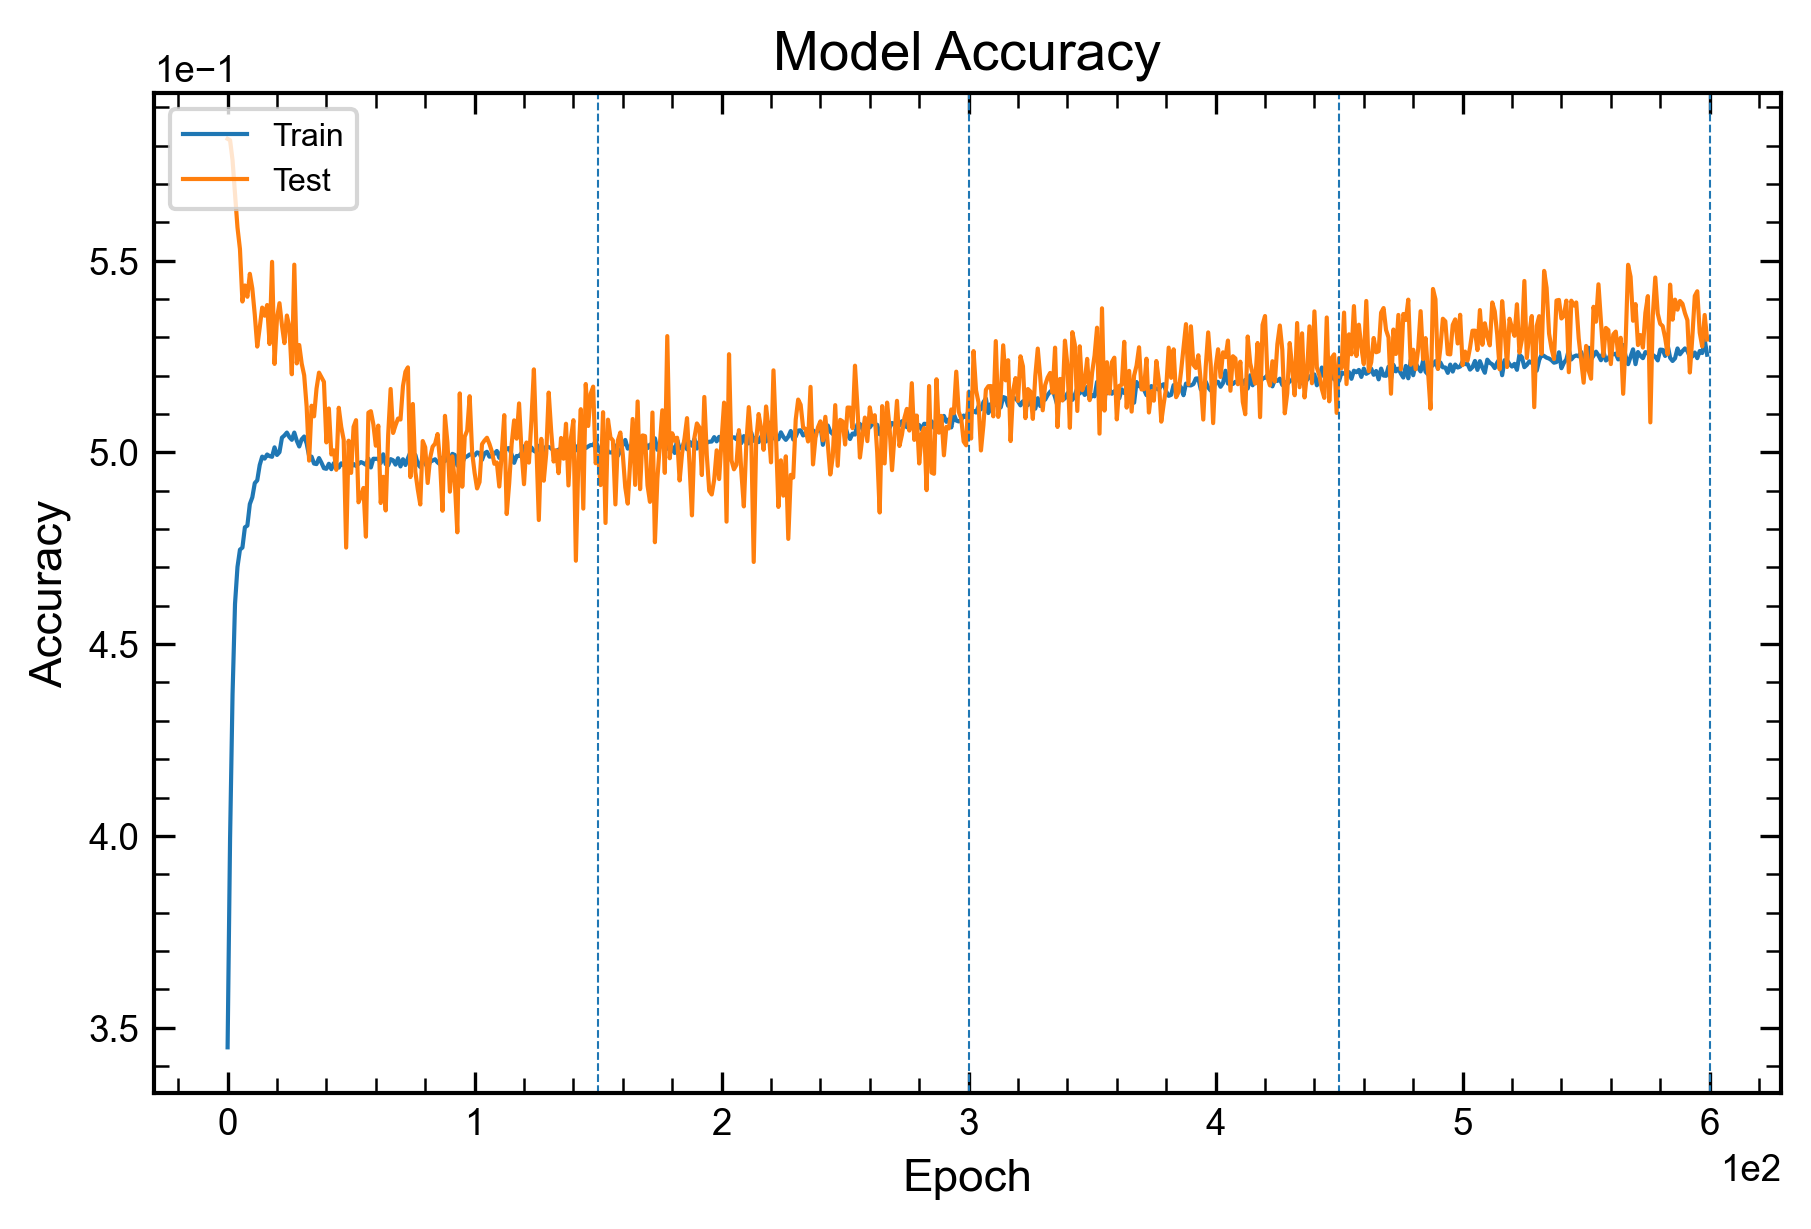
\includegraphics[width=\textwidth]{acc_lephad.png}
    \end{figure}
  \end{column}
\end{columns}
\end{frame}

\begin{frame}{Results hadhad}
\begin{columns}
  \begin{column}{0.5\textwidth}
    \begin{figure}
      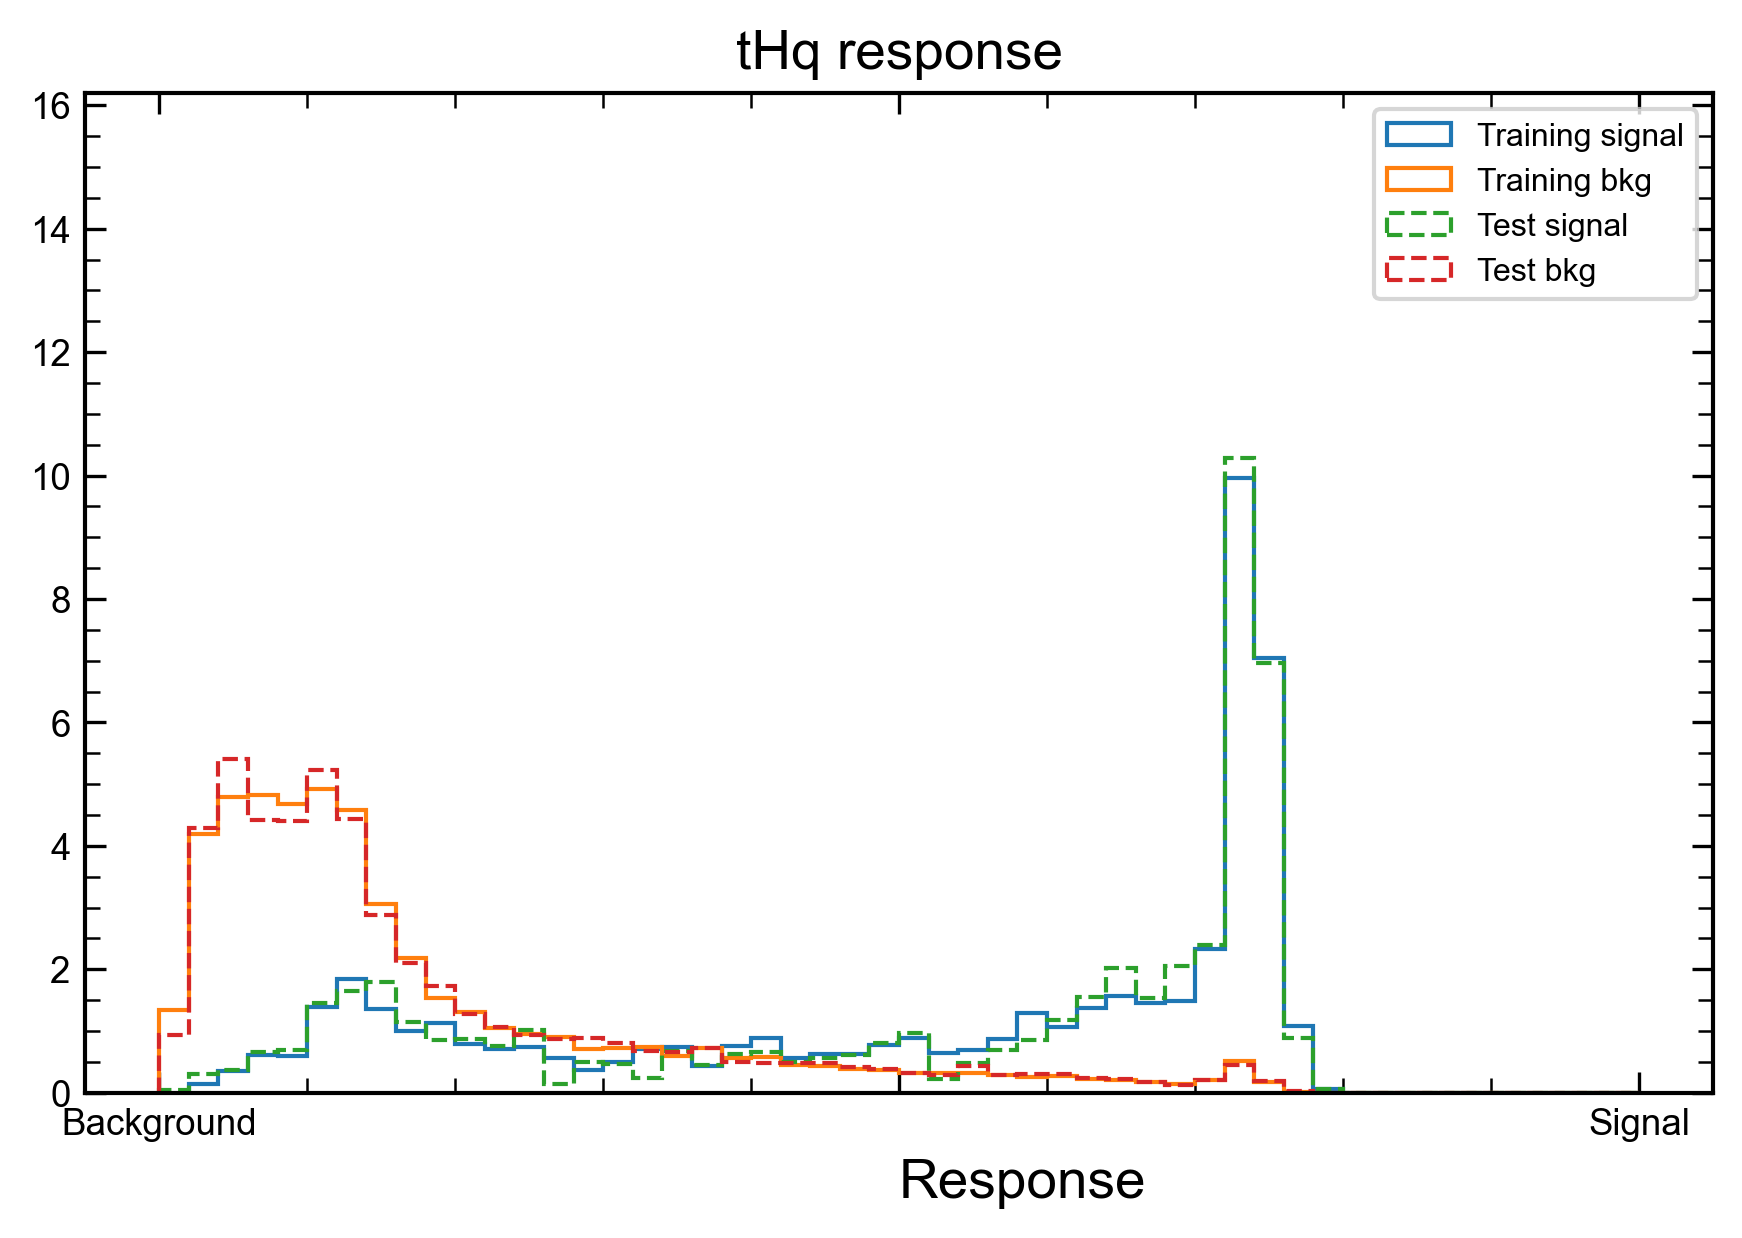
\includegraphics[width=\textwidth]{response_lephad.png}
    \end{figure}
  \end{column}
  \begin{column}{0.5\textwidth}
    \begin{figure}
      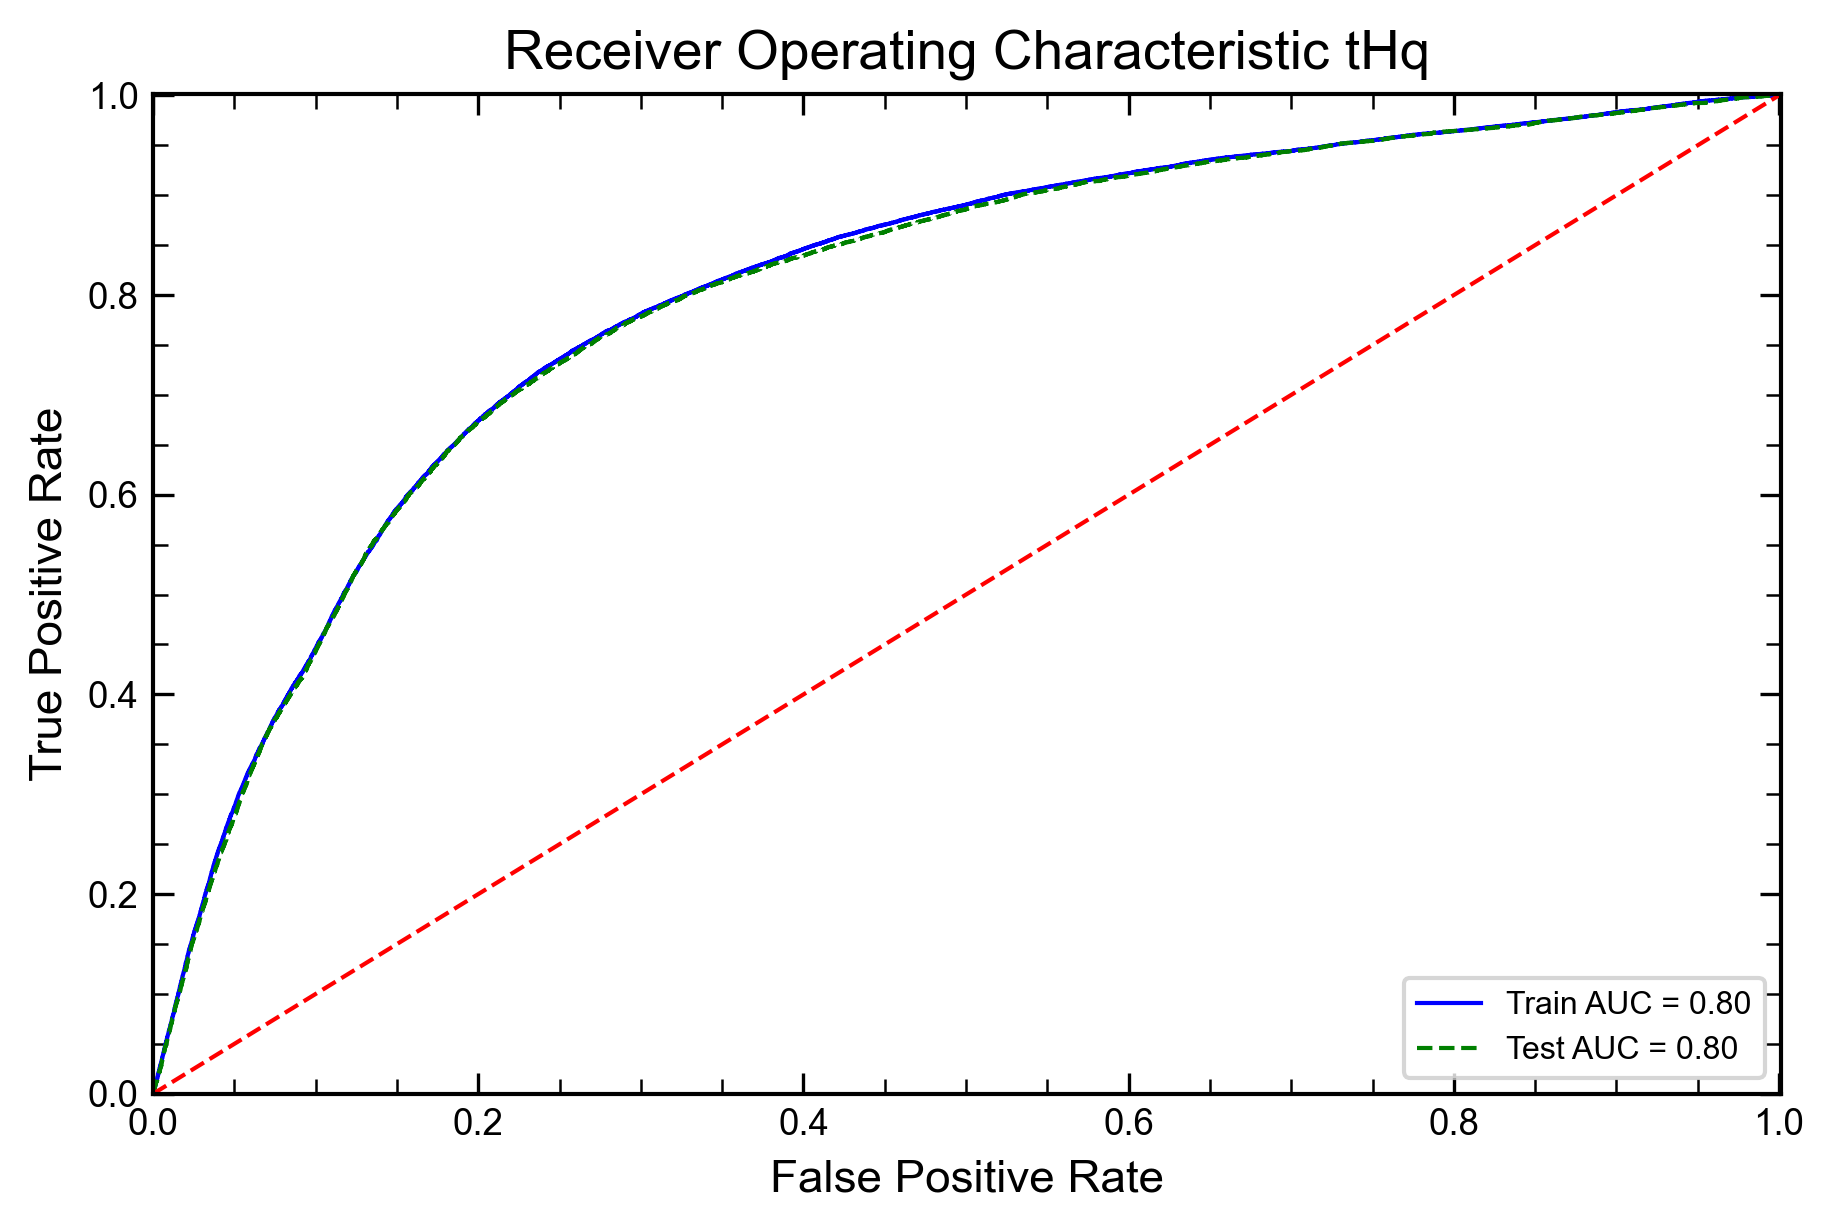
\includegraphics[width=\textwidth]{ROC_lephad.png}
    \end{figure}
  \end{column}
\end{columns}
\end{frame}